\documentclass{article}
\usepackage{amsmath} % Required for typesetting matrices
\usepackage{amssymb} % Required for using the "therefore" symbol
\usepackage{graphicx}

\title{Matrix, Linear Algebra, Differential Equation \\ MAT 2207}
\author{Jannat Tohfa Chowdhury}
\date{April 2024}

\begin{document}
\maketitle
\newpage
% Your lectures start here
\section*{Matrix}
\subsection*{Definition of Matrix: }
\vspace{10pt}
A system of any \( m \times n \) numbers arranged in a rectangular arrangement of \( m \) rows and \( n \) columns is called a matrix of order \( m \times n \) or an \( m \times n \) matrix.
    \paragraph{Ex:}
    \[
    \begin{minipage}{0.6\textwidth}
    \[
    \begin{bmatrix}
    1 & -2 & 4 \\
    3 & 1 & 7 \\
    \end{bmatrix}
    \]
    \end{minipage}
    \begin{minipage}{0.4\textwidth}
    is a $2 \times 3$ matrix.
    \end{minipage}
    \]
    \vspace{12pt}
    \textbf{in general form:}
    \[
    A = 
    \begin{bmatrix}
    \sigma_{11} & \sigma_{12} & \cdots & \sigma_{1n} \\
    \sigma_{21} & \sigma_{22} & \cdots & \sigma_{2n} \\
    \vdots & \vdots & \vdots & \vdots \\
    \sigma_{m1} & \sigma_{m2} & \cdots & \sigma_{mm}
    \end{bmatrix}
    =(\sigma_{ij})_{mxm}
    \]
\vspace{20pt}
\subsection*{Singular and Non-singular Matrix:}
\vspace{10pt}
    Let \( A \) be any square matrix. If \( \det(A) = 0 \), then \( A \) is called a singular matrix, and if \( \det(A) \neq 0 \), then \( A \) is called a non-singular matrix.
    \vspace{12pt}
    \paragraph{Ex:}
    \begin{minipage}{0.4\textwidth}
    \[ A = 
    \begin{bmatrix}
    1 & 2 \\
    2 & 4 \\
    \end{bmatrix} \]
    \end{minipage}
    \begin{minipage}{0.1\textwidth}
    \end{minipage} 
    \begin{minipage}{0.4\textwidth}
    \[ B = 
    \begin{bmatrix}
    1 & 5 \\
    2 & 12 \\
    \end{bmatrix} \]
    \end{minipage}

    \vspace{20pt}    
    Then \(|A| = \det(A) = \det \begin{bmatrix} 1 & 2 \\ 2 & 4 \end{bmatrix} = 4 - 4 = 0\)
    
    So, \(A\) is a singular matrix
    
    \vspace{20pt}
    Again, \(|B| = \det(B) = \det \begin{bmatrix} 1 & 5 \\ 2 & 12 \end{bmatrix} = 12 - 10 = 2 \neq 0\)
    
    Hence, \( B \) is a non-singular matrix.
\vspace{20pt}
\subsection*{Inverse Matrix:}
\vspace{10pt}
    Let \( A \) and \( B \) be two \(n \times n\) square matrices such that \( AB = BA = I_{n} = I \), then \( B \) is said to be the inverse of \( A \), and we write \( B = A^{-1} \). Also, \( A = B^{-1} \).
    \vspace{20pt}
    \paragraph{Ex:}
    Let \( A = \begin{bmatrix} 4 & 3 \\ 1 & 1 \end{bmatrix} \) and \( B = \begin{bmatrix} 1 & -3 \\ -1 & 4 \end{bmatrix} \).
    
    \vspace{10pt}
    
    \begin{minipage}{.45\textwidth}
    \(\therefore\ AB = 
    \begin{bmatrix} 4 & 3 \\ 1 & 1 \end{bmatrix}
    \times
    \begin{bmatrix} 1 & -3 \\ -1 & 4 \end{bmatrix}\)
    \end{minipage}

    
    \vspace{10pt}
    
    \begin{minipage}{0.7\textwidth}
    \[ = \begin{bmatrix} 4 - 3 & -12 + 12 \\ 1 - 1 & -3 + 4 \end{bmatrix} = \begin{bmatrix} 1 & 0 \\ 0 & 1 \end{bmatrix} = I_{2} \]
    \end{minipage}
    
    \vspace{10pt}
    
    \begin{minipage}{0.6\textwidth}
    and \( BA = \begin{bmatrix} 1 & -3 \\ -1 & 4 \end{bmatrix} \times \begin{bmatrix} 4 & 3 \\ 1 & 1 \end{bmatrix} \)
    \end{minipage}
    
    \vspace{10pt}

    \begin{minipage}{0.7\textwidth}
        \[ = \begin{bmatrix} 4 - 3 & 3 - 3 \\ -4 + 4 & -3 + 4 \end{bmatrix} = \begin{bmatrix} 1 & 0 \\ 0 & 1 \end{bmatrix} = I_{2} \]
    \end{minipage}
   
    \vspace{10pt}
    
    \(\therefore\)\(AB = BA = I_{2} = I\)
    
    Therefore, we can write \( A = B^{-1} \) and \( B = A^{-1} \).

    \vspace{30pt}
    [N.B.: The inverse of a matrix exists only when the matrix is non-singular,

i.e., \( |A| \neq \emptyset \).]

    *** Multiplication of two matrices is possible only when the number of columns in the first matrix is equal to the number of rows in the second matrix.

\vspace{20pt}

\subsection*{Echelon Matrix:}
    \vspace{10pt}
    Let \( A = (a_{ij})_{m \times n} \) be any matrix. Then \( A \) is said to be an echelon matrix or is said to be in echelon form if:
    \begin{enumerate}
        \item all the non-zero rows (if any) precede the zero rows,
        \item the number of zero entries preceding the first non-zero entry in each row increases by row.
    \end{enumerate}

    \vspace{10pt}

    \paragraph{Ex:}
    \[\begin{bmatrix} 1 & -1 & 2 \\ 0 & 3 & 2 \\ 0 & 0 & 5 \end{bmatrix} \text{ is an echelon matrix,  but } \begin{bmatrix} 1 & 2 & 3 \\ 0 & -1 & 3 \\ 2 & 5 & 4 \end{bmatrix} \text{ is not an echelon matrix.}\]

    \vspace{20px}

\subsection*{Rank of a Matrix:}
    \vspace{10pt}
    Rank of a matrix is the largest non-zero row in the matrix of row echelon form.

    \paragraph{Ex:}
    \begin{minipage}{0.45\textwidth}
    \[ A = \begin{bmatrix} 1 & 4 & 5 \\ 0 & 3 & 7 \\ 0 & 0 & 6 \end{bmatrix} \]
    \end{minipage}
    \begin{minipage}{0.45\textwidth}
        \[ B = \begin{bmatrix} 1 & 2 & 3 \\ 0 & 6 & 7 \\ 0 & 0 & 0 \end{bmatrix} \]
    \end{minipage}

    \vspace{20pt}
    \text{Rank of matrix } A = 3, \quad \text{Rank of matrix } B = 2

    \vspace{60pt}
    \textbf{Find the rank of the following matrices:}
    
    \begin{center}
    \begin{minipage}{0.45\textwidth}
    \[ A = \begin{bmatrix} 1 & -1 & -1 & 2 \\ 2 & 1 & 3 & -1 \\ 3 & 2 & 1 & 2 \\ 4 & 1 & 2 & 3 \end{bmatrix} \]
    \end{minipage}
    \hspace{0.05\textwidth}
    \begin{minipage}{0.45\textwidth}
    \[ B = \begin{bmatrix} 1 & 3 & 1 & -2 & -3 \\ 1 & 4 & 3 & -1 & -4 \\ 2 & 3 & -4 & -7 & -3 \\ 3 & 8 & 1 & -7 & -8 \end{bmatrix} \]
    \end{minipage}
    \end{center}
    
    \vspace{1em}
    
    \begin{center}
    \begin{minipage}{0.45\textwidth}
    \[ C = \begin{bmatrix} 1 & -1 & 2 & 1 \\ 3 & 0 & 2 & 2 \\ 2 & 1 & -1 & 1 \\ 1 & 0 & 1 & 1 \end{bmatrix} \]
    \end{minipage}
    \hspace{0.05\textwidth}
    \begin{minipage}{0.45\textwidth}
    \[ D = \begin{bmatrix} 1 & -1 & 1 & 3 \\ 2 & -1 & 0 & 2 \\ 1 & 0 & 1 & 1 \\ 4 & 2 & 0 & 1 \end{bmatrix} \]
    \end{minipage}
    \end{center}

    \vspace{120pt}

    \begin{figure}[htbp]
        \centering
        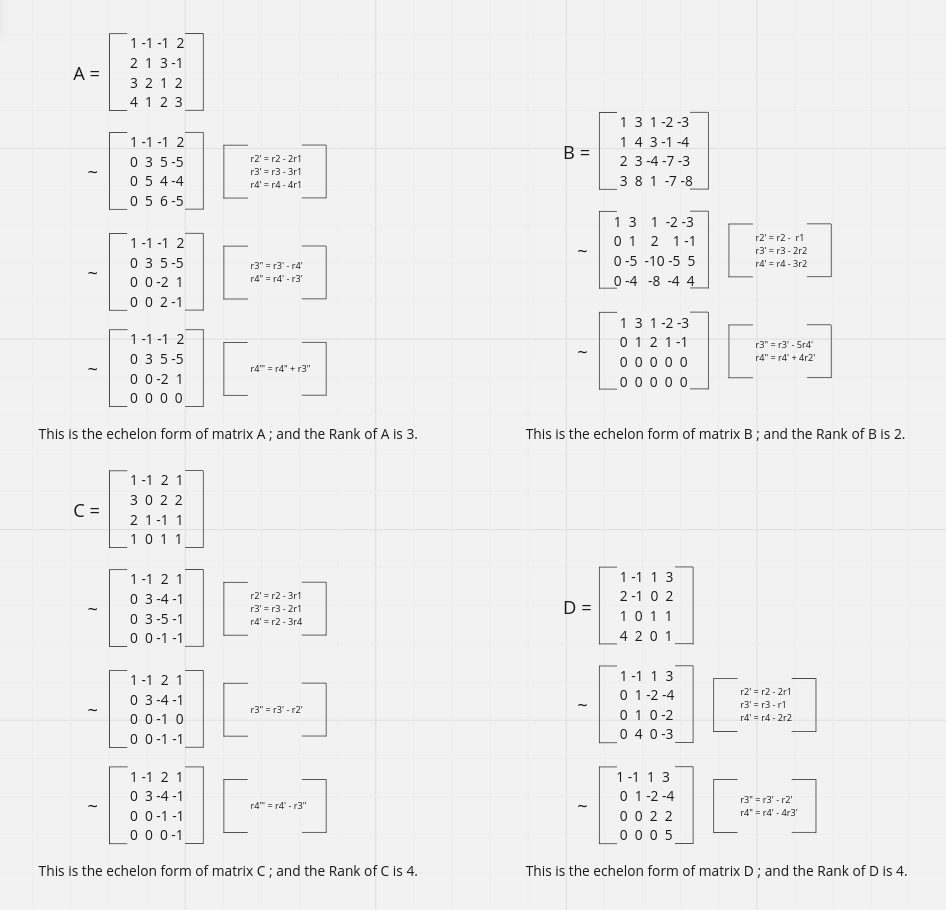
\includegraphics[width=1.2\textwidth, height=.95\textheight]{../asset/rankOfExc.png}
        \label{fig:example}
    \end{figure}
    
    \newpage
    \section*{Inverse Matrix Calculation:}
    \vspace{10pt}
    Find the inverse of the matrix by using the formula [A:I]

    \vspace{10pt}
    example; find the inverse matrix of \( A = \begin{bmatrix} 1 & -1 & 2 & 1 \\ 3 & 0 & 2 & 2 \\ 2 & 1 & -1 & 1 \\ 1 & 0 & 1 & 1 \end{bmatrix} \)

    \vspace{10pt}
    Solution:
    \vspace{10pt}
    \begin{figure}[htbp]
        \centering
        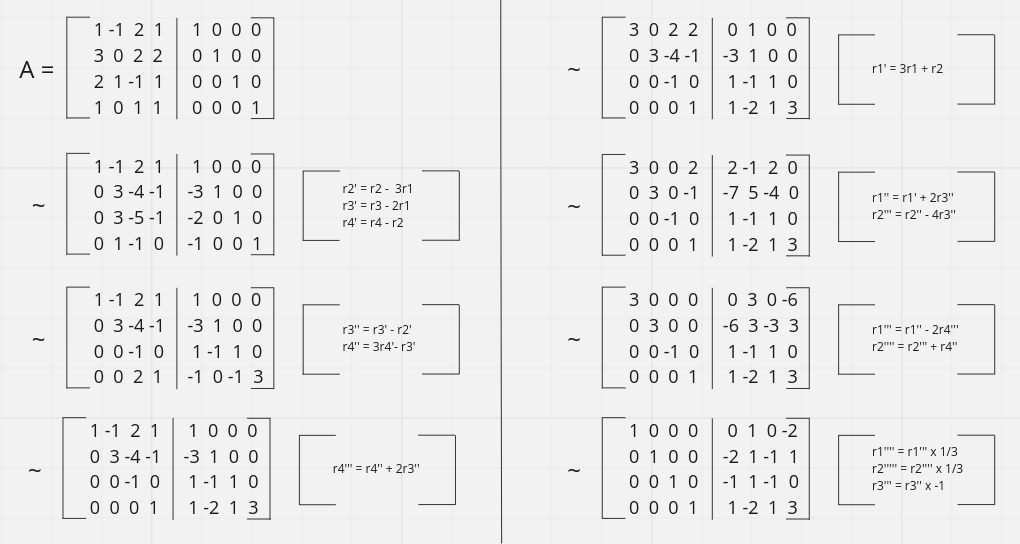
\includegraphics[width=1.2\textwidth, height=.7\textheight]{../asset/invEXA.png}        \label{fig:example}
    \end{figure}

    \vspace{10pt}
    \newpage
    \underbar{Home Work:}

    find the inverse matrix of
    \hspace*{10pt}
    \( B = \begin{bmatrix} -1 & 2 & -3 \\ 2 & 1 & 0 \\ 4 & -2 & 5 \end{bmatrix} \);  
    \( C = \begin{bmatrix} 1 & 3 & 1 & 1 \\ 2 & 5 & 2 & 2 \\ 1 & 3 & 8 & 9 \\ 1 & 3 & 2 & 2 \end{bmatrix} \)
    
    \begin{figure}[htbp]
        \centering
        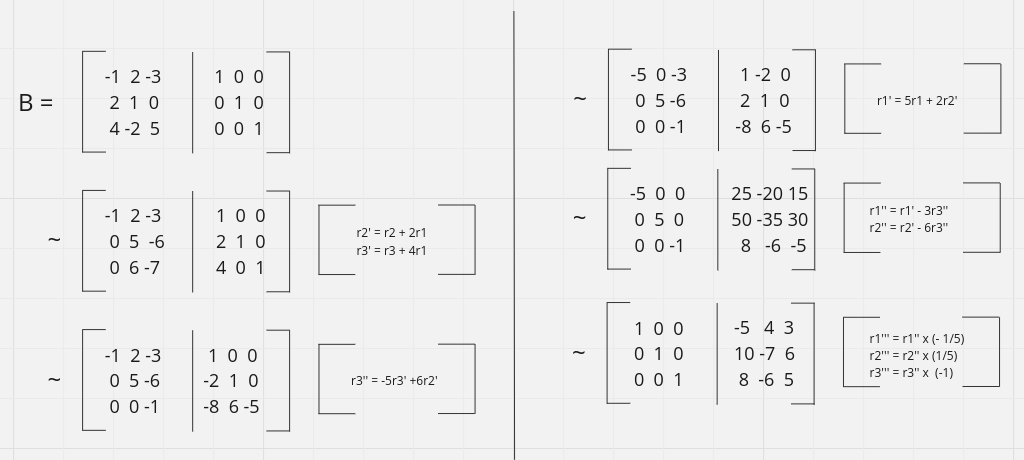
\includegraphics[width=1.2\textwidth, height=.7\textheight]{../asset/invHWB.png}
        \label{fig:example}
    \end{figure}
    \begin{figure}[htbp]
        \centering
        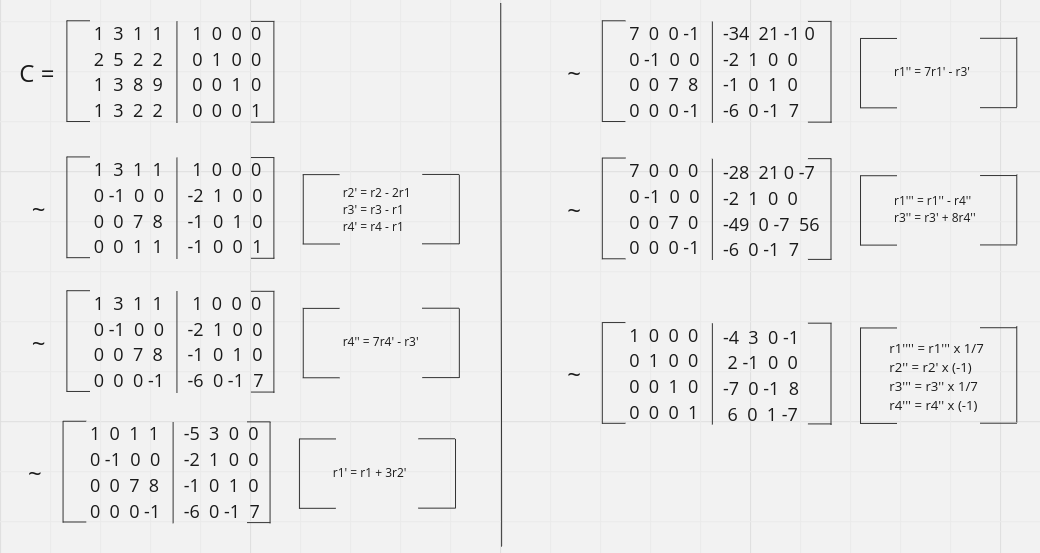
\includegraphics[width=1.2\textwidth, height=.7\textheight]{../asset/invHWC.png}
        \label{fig:example}
    \end{figure}

    \newpage

    \end{document}


